\documentclass{litesolution}
\usepackage[level]{datetime}

\makeatletter
\definecolor{pkgcolor}{Hsb}{103,.8,.5}
\definecolor{moducolor}{Hsb}{290,.8,.5}
\definecolor{cmdcolor}{Hsb}{188,.8,.5}
\definecolor{filecolor}{Hsb}{207,.6,.7}
\definecolor{H1}{Hsb}{349,.8,.8}% 海棠紅 (Hangzhou MTR L 1 )
\definecolor{H2}{Hsb}{23, .8,.8}% 丹桂橙 (Hangzhou Metro 2 )
\definecolor{H3}{Hsb}{48, .8,.8}% 柠檬黄 (Hangzhou Metro 3 )
\definecolor{H4}{Hsb}{103,.8,.8}% 香樟绿 (Hangzhou Metro 4 )
\definecolor{H5}{Hsb}{188,.8,.8}% 青藍色 (Hangzhou MTR L 5 )
\definecolor{H6}{Hsb}{207,.8,.8}% 海洋蓝 (Hangzhou Metro 6 )
\definecolor{H7}{Hsb}{290,.8,.8}% 浪漫紫 (Hangzhou Metro 7 )
\hypersetup{colorlinks,urlcolor=H1,linkcolor=H2,filecolor=filecolor,pdfstartview=FitH,pdfview=FitH,pdfcreator=XeTeX output}

\def\@pkg#1{\texorpdfstring{\href{https://www.ctan.org/pkg/#1}{\textcolor{pkgcolor}{\textsf{#1}}}}{“#1”}}
\def\s@pkg#1{\texorpdfstring{\textcolor{pkgcolor}{\textsf{#1}}}{“#1”}}
\DeclareRobustCommand\pkg{\@ifstar\s@pkg\@pkg}
\def\mode#1{\texorpdfstring{\textcolor{moducolor}{\textsf{#1}}}{“#1”}}
\def\cmd#1{\texorpdfstring{\textcolor{cmdcolor}{\textsf{#1}}}{“#1”}}
\def\datechange#1#2{%
  \noindent{\makebox[\textwidth][r]{\color{H7}\rule{1.15\textwidth}{.4pt}}}
  \noindent\makebox[0pt][r]{\makebox[-3em][r]{\small\textbf{\textcolor{H7}{#1}}}\;\;}{\sffamily Update: \ignorespaces#2}}
\makeatother

% \watermark{ctanlion}

\begin{document}

\chapterimage{cover1.png}
\chapter{The \pkg{LiteSolution} Template}
\fancyhead[L]{\,\color{H7}\href{https://github.com/xiamyphys/litesolution}{\faIcon{github}\;\leftmark}}
\fancyhead[R]{\color{H7}\rightmark\,}

\centerline{Xia Mingyu, \href{https://www.hdu.edu.cn}{Hangzhou Dianzi University}}
\ddmmyyyydate
\centerline{\mailto{xiamyphys@gmail.com}}
\centerline{\today,\quad Version 1.0a}

This is the document for \pkg{LiteSolution} template, which provides a lite design of the solution of test paper.

Some designs of this template currently only support \textbf{Simplified Chinese (Mainland)}. If necessary, you can change some Chinese characters to the language you want in the \verb|*.cls| file.

\section{Introduction}
\subsection{The purpose of this template}
This template provides a lite and fresh template, and mainly used for typesetting solutions of final, textbooks' and other exercises. This template is developed based on ElegantBook, ported and improved the chapter design module code of \href{https://www.overleaf.com/latex/templates/the-legrand-orange-book-template-english/jtctyfmnpppc}{The Legrand Orange Book}. I'd like to express my gratitude to the two template authors for their previous work.

If you meet bugs when using this template, or you have better suggestions or ideas, or you want to participate in the development of the template or other templates by me, welcome to contact via email \href{mailto:xiamyphys@gmail.com}{xiamyphys@gmail.com}.

Also, you can join my \textsf\LaTeX{} Template Discussion \href{https://qm.qq.com/q/OnHzbNvVAG}{QQ Group: 760570712} to communicate with me and get the insider preview edition of the template.

\section{Modes of \pkg{LiteSolution}}
\subsection{The \mode{answer} mode}
These two modes \mode{ans} and \mode{noans} can show and hide answers respectively. After you choose the \mode{noans}, the contents in the environment \cmd{solution}, the command \cmd{ans} and the answers in the multiple choice questions will all become the same color as the pagecolor. So the area that originally contained the answer will be replaced by an area of the same blank size. You can generate exams without answers and solutions by enabling \mode{noans}.

\subsection{The \mode{mtpro2} mode}
If you've installed the \emph{Mathtime Pro 2 Lite} font in your computer, then you can use this mode to change the formula font in the test paper.
\subsection{The \mode{separate} and \mode{continuous} modes}
You can insert multiple test questions into one document. The page numbers between each test question will be continuous when you use the \mode{continuous} mode or the page number of each test question will start from 1 when you use the \mode{separate}.


\section{Commands of \pkg{LiteSolution}}
\subsection{The \cmd{chapterimage} command}
\begin{verbatim}
    \chapterimage{cover1.png}
\end{verbatim}
This command can assign the title background image for each subsequent chapter.

\subsection{The \cmd{chapterfont} command}
This command can assign the title font for each subsequent chapter, if you do not use this command, the title font will be \emph{songti} in Chinese and \emph{Libertinus} in English.

\subsection{The \cmd{ans} command}
This command can underlines the answer and changes the color of the answer to \textcolor{1号色}{Blue Sapphire}.

\paragraph{If mode \mode{noans} is enabled, the answer will disappear, leaving only a horizontal line the same width as the answer.}

\subsection{The \cmd{watermark} command}
\begin{verbatim}
    \watermark{ctanlion.pdf}
\end{verbatim}

This command can add watermark to the document.

\subsection{Other customer commands}
In order to facilitate input, the following commands are scheduled. You can add others in the \verb|*.cls| file as you like.
\vskip1em
\begin{center}
    \begin{tabular}{l|l|l|l|l|l}
        \toprule
        Command & Output & Command & Output & Command & Output\\
        \midrule
        \verb|\titlelogo{#1}{#2}| & Add emoji with link in text & \verb|\point{#1}| & Add score & \verb|\i| & $\mathrm{i}$\\
        \hline
        \verb|\sokka{#1}| & 故本题选择\#1项 & \verb|\d| & $\mathrm{d}$ & \verb|\e| & $\mathrm{e}$\\
        \bottomrule
    \end{tabular}    
\end{center}

\section{Environments of \pkg{LiteSolution}}
\subsection{The \cmd{choice} environment}
There're two variables in this envrionment. The first one is the answer of the choice problem, the second one is the keywords of this choice problem and it's optional.

\begin{tcblisting}{sidebyside}
\begin{choice}{D}[Keywords]
If you want to add choice and keywords.
\begin{tasks}(2) % 2 choices per line
    \task This is choice A  \task This is choice B
    \task This is choice C  \task This is choice D
\end{tasks}
\end{choice}
\begin{choice}{D}
If you want to add choice only.
\begin{tasks}(4) % 4 choices per line
    \task Chc A \task Chc B \task Chc C \task Chc D
\end{tasks}
\end{choice}
\end{tcblisting}

\begin{paracol}{2}
    \begin{choice}{D}[Gaussian theory]
        $A$和$B$为两个均匀带电球体,$A$带电荷$+q$,$B$带电荷$-q$,作一与$A$...
        \begin{tasks}(2)
            \task 通过$S$面的电场强度...        \task 通过$S$面的电场强度...
            \task 通过$S$面的电场强度...        \task 通过$S$面的电场强度...
        \end{tasks}
    \end{choice}
    \switchcolumn
    \centering\vfill
    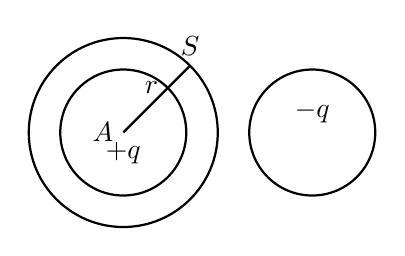
\begin{tikzpicture}
        \draw [thick] (0,0) circle (0.8);
        \draw [thick] (0,0) circle (1.2);
        \draw [thick] (2.4,0) circle (0.8);
        \draw [thick] (0,0)--(0.85,0.85);
        \node [anchor=east] at (0,0) {$A$};
        \node [anchor=north] at (0,0) {$+q$};
        \node [anchor=east] at (0.566,0.566) {$r$};
        \node [anchor=south] at (0.85,0.85) {$S$};
        \node [anchor=south] at (2.4,0) {$-q$};
    \end{tikzpicture}
    \vfill
\end{paracol}
\begin{verbatim}
\begin{paracol}{2}
\begin{choice}{D}[Gaussian theory]
    $A$和$B$为两个均匀带电球体,$A$带电荷$+q$,$B$带电荷$-q$,作一与$A$...
    \begin{tasks}(2)
        \task 通过$S$面的电场强度...        \task 通过$S$面的电场强度...
        \task 通过$S$面的电场强度...        \task 通过$S$面的电场强度...
    \end{tasks}
\end{choice}
\switchcolumn\centering\vfill\tikz{...}\vfill
\end{paracol}
\end{verbatim}

\subsection{The \cmd{problem} environment}
Sightly different from the cmd{choice} environment: the two variables are points and keywords, and the question number counter is shared with the multiple-choice question number counter.
\begin{tcblisting}{sidebyside}
    \begin{problem}[Keywords][5]
        If you want to add keywords and points.
    \end{problem}
    \begin{problem}
        If you want to add none.
    \end{problem}
    \begin{problem}[Keywords]
        If you want to add keywords only.
    \end{problem}
    \begin{problem}*[][5]
        If you want to add points only.
    \end{problem}
\end{tcblisting}

\begin{paracol}{2}
\begin{problem}[Gaussian theory \& Field strength][6]
    一均匀带电直导线长为$d$,电荷线密度为$+\lambda$.过导线中点$O$作一半径为$R$($R>\frac{d}{2}$)的球面$S$,$P$为带电直导线的延长线与球面$S$的交点. 则通过该球面的电场强度通量$\Phi_e=$\ans{$\frac{\lambda d}{\varepsilon_0}$},带电直线的延长线与球面交点$P$处的电场强度的大小为\ans{$\frac{\lambda d}{4\pi\varepsilon_0(R^2-d^2/4)}$},方向\ans{沿矢径$\boldsymbol{OP}$}.
    \end{problem}
\switchcolumn\centering
\vfill
\begin{tikzpicture}[scale=0.83]
    \draw (0,0) circle (2);
    \draw [thick,->] (-2,0)--(0,0)--(1,1.732);
    \node [anchor=east] at (-2,0) {$P$};
    \filldraw (-2,0) circle (0.05);
    \node [anchor=west] at (0.5,0.866) {$R$};
    \filldraw [pattern=north east lines] (-0.8,-0.1)--(-0.8,0.1)--(0.8,0.1)--(0.8,-0.1)--cycle;
    \draw [thick,|<-] (-0.8,-0.3)--(-0.25,-0.3);
    \draw [thick,|<-] (0.8,-0.3)--(0.25,-0.3);
    \node at (0,-0.3) {$L$};
\end{tikzpicture}
\vfill
\end{paracol}
\begin{verbatim}
\begin{paracol}{2}
    \begin{problem}[Gaussian theory \& Field strength][6]
        一均匀带电直导线长为$d$,电荷线密度为$+\lambda$,过导线中点$O$...
        场强大小\ans{$\frac{\lambda d}{4\pi\varepsilon_0(R^2-d^2/4)}$}...
    \end{problem}
\switchcolumn\centering\vfill\tikz{...}\vfill
\end{paracol}
\end{verbatim}

\subsection{The \cmd{note} environment}
\begin{tcblisting}{sidebyside}
\begin{note}
    Please note that...
\end{note}
\end{tcblisting}

\subsection{The \cmd{solution} environment}
\begin{tcblisting}{sidebyside}
\begin{solution}
    This is the answer for the problem.
\end{solution}
\end{tcblisting}

If a star (*) is added after the \verb|\begin{solution}|, then the content will follow the 
\begin{tcblisting}{sidebyside}
\begin{solution}*
    This is the answer for the problem.
\end{solution}
\end{tcblisting}

\paragraph{If mode \mode{noans} is enabled, the solution will disappear, leaving only a blank box with the same height as the solution, and the name of the box will change to \emph{\textcolor{1号色}{\textbf{\faIcon{ban} 答案隐藏}}}.}

\section{Version History}

\textsf{\bfseries Version 0.1a} was finished developing on 29 June, 2023. 

\textsf{\bfseries Version 0.1b} was finished developing on 6 July, 2023 and released on \href{https://www.latexstudio.net/index/details/index/mid/3553.html}{LaTeX Studio} (Xiaoshan, Hangzhou) and \href{http://xhslink.com/YBuuuw}{Xiaohongshu}, where won the favor of many people and even some people.

\datechange{06/07/2023}{Version 0.1b}
\begin{itemize}
    \item Support page number remaking between chapters.
    \item Added \cmd{watermark} command.
\end{itemize}

\datechange{15/11/2023}{Version 1.0a}
\begin{itemize}
    \item Redesigned the \cmd{chapterimage} part, include the layout and the code.
    \item Redesigned the \cmd{choice} environment, supports not adding keywords.
    \item Deleted the \cmd{exercise} environment, replaced with the \cmd{problem} environment, supports adding only keywords or points.
    \item Redesigned the \cmd{solution} environment, supports star (*) key. 
    \item Added the \cmd{note} environment and some customer commands.
\end{itemize}
\chapter{A Sample for \pkg{LiteSolution} Template}
\fancyhead[L]{\color{H6}\kaishu\faIcon{atom}\;2023年\titlelogo{https://sci.hdu.edu.cn}{HDU}「大学物理2」期中模拟}
\fancyhead[R]{\color{H6}\kaishu\rightmark\,}

\section{选填题(共15分)}
\begin{choice}{D}[波的能量]
    一平面简谐波在弹性媒介中传播,在媒质质元从最大位移处回到平衡位置的过程中
    \begin{tasks}(2)
        \task 它的势能转换成动能
        \task 它的动能转换成势能
        \task 它从相邻的一段质元获得能量,其能量逐渐增加
        \task 它把能量传给相邻的一段质元,其能量逐渐减小
    \end{tasks}
\end{choice}
\begin{solution}*
    波在传播过程中介质质元振动的动能和势能同时变化.\sokka{C}
\end{solution}

\begin{choice}{D}[双缝干涉]
    在双缝干涉实验中,两缝间距离为$d$,双缝与屏幕之间的距离为$D$($D\gg d$).波长为$\lambda$的平行单色光垂直照射到双缝上,屏幕上干涉条纹中相邻暗纹之间的距离是
    \begin{tasks}(4)
        \task $\frac{2\lambda D}{d}$
        \task $\frac{\lambda d}{D}$
        \task $\frac{dD}{\lambda}$
        \task $\frac{\lambda D}{d}$
    \end{tasks}
\end{choice}
\begin{solution}*
    由明纹公式$x=k\lambda D/d$得暗纹间距$\Delta x=\lambda D/d$.\sokka{D}
\end{solution}

\begin{problem}[简谐振动的合成][3]
    一个质点同时参与两个在同一直线上的简谐振动:$x_1=4\cos{(2t+\frac{\pi}{6})},\ x_2=2\cos{(2t-\frac{\pi}{6})}$.该质点合振动的振幅大小为\ans{$2\sqrt{7}$}.
\end{problem}
\begin{solution}*
    $A=\sqrt{A_1^2+A_2^2+2A_1A_2\cos{\Delta\varphi}}=2\sqrt{7}$.
\end{solution}

\begin{problem}[多普勒效应][6]
    一辆运动的警车发出警铃声音频率为$f_s=1400\mathrm{Hz}$,从左向右移动,速度大小为$70\mathrm{m/s}$. 一个观察者从右向左移动,速度大小为$10\mathrm{m/s}$,空气中的声速$u=340\mathrm{m/s}$.观察者与警车相遇前后,听到警铃的频率分别为\ans{$1814.8\mathrm{Hz}$,$1126.8\mathrm{Hz}$}.
\end{problem}
\begin{solution}*
    $f_1=\frac{340+10}{340-70}\times 1400\mathrm{Hz}\approx 1814.8\mathrm{Hz},\ f_2=\frac{340-10}{340+70}\times 1400\mathrm{Hz}\approx 1126.8\mathrm{Hz}$.
\end{solution}

\section{计算题(共20分)}
\begin{problem}[简谐振动][10]
    一个质量为$1\mathrm{kg}$的物块沿$x$轴做简谐振动,振幅为$10\mathrm{cm}$,最大速度$2\times 10^{-2}\mathrm{m/s}$.在时间$t=4\mathrm{s}$时,物块位于$5\mathrm{cm}$.求
    \begin{enumerate}
        \item 简谐运动的周期和最大加速度.
        \item 简谐运动的位移方程.
    \end{enumerate}
\end{problem}
\begin{solution}
    \begin{enumerate}
        \item 由$v_{\max}=\omega,\ T=\frac{2\pi}{\omega}$得$T=10\pi\mathrm{s},\ \omega=0.2\mathrm{s}^{-1},\ a_{\max}=\omega^2A=4\times 10^{-3}\mathrm{m/s}^2$.\point{4}
        \item $t=4\mathrm{s}$时$x=\frac{1}{2}A,\ v<0$,所以此时相位$\varphi=\frac{\pi}{3}$.故位移方程为\point{2}
        \[x=0.1\cos{[0.2(t-4)]+\frac{\pi}{3}}=0.1\cos{(0.2t+0.079\pi)}\eqno\point{4}\]
    \end{enumerate}
\end{solution}

\begin{problem}[牛顿环][10]
    空气中,使用波长为$480\mathrm{nm}$平行单色光观察牛顿环.在反射光中测得某一明环的直径为$4.74\mathrm{mm}$,在它外面第$10$个明环的直径为$7.24\mathrm{mm}$.求
\begin{enumerate}
    \item 平凸透镜的曲率半径.
    \item 直径为$4.74\mathrm{mm}$明环的条纹级数$k$.
    \item 假设把整个装置放入水中($n=1.33$),原直径为$4.74\mathrm{mm}$明环的新直径.
\end{enumerate}
\end{problem}
\begin{solution}
\begin{enumerate}
    \item $R=(r_{k+10}^2-r_k^2)/10\lambda=1.56\mathrm{m}$.\point{4}
    \item 由$r_k=\sqrt{\frac{2k-1}{2}\lambda R}$得$k=\frac{r_k^2}{\lambda R}+\frac{1}{2}=8$.\point{3}
    \item 由于光在介质中的波长与折射率成反比,所以此时$d_k^{\prime}=\frac{d_k}{\sqrt{n}}=4.11\mathrm{mm}$.\point{3}
\end{enumerate}
\end{solution}

\section{计算题\! $^\dagger$(共15分)}

\begin{problem}[弹簧振子][15]
    一个质量为$m=1\mathrm{kg}$的盘子刚性连接竖直悬挂的轻弹簧下端,弹簧的劲度系数为$k=90\mathrm{N/m}$.盘子在竖直方向做简谐运动,振幅$A=10.0\mathrm{cm}$.现有一个质量$m_2=1\mathrm{kg}$的物体自由落下掉在盘上,没有反弹.当\textbf{盘子位于向上最大位移处},盘子与物体发生碰撞,物体从开始自由自由落体发生处,距离为$h=20\mathrm{cm}$,假设碰撞瞬间完成.求碰撞后盘子和物体组成的系统,它的振动周期、振幅和振动能量.
\end{problem}
\begin{solution}*
    Answer omitted.
\end{solution}
\end{document}